\documentclass[journal,12pt,twocolumn]{IEEEtran}

\usepackage{setspace}
\usepackage{gensymb}
\singlespacing
\usepackage[cmex10]{amsmath}

\usepackage{amsthm}

\usepackage{mathrsfs}
\usepackage{txfonts}
\usepackage{stfloats}
\usepackage{bm}
\usepackage{cite}
\usepackage{cases}
\usepackage{subfig}
\usepackage{graphicx}
\usepackage{longtable}
\usepackage{multirow}

\usepackage{enumitem}
\usepackage{mathtools}
\usepackage{steinmetz}
\usepackage{tikz}
\usepackage{circuitikz}
\usepackage{verbatim}
\usepackage{tfrupee}
\usepackage[breaklinks=true]{hyperref}
\usepackage{graphicx}
\usepackage{tkz-euclide}

\usetikzlibrary{calc,math}
\usepackage{listings}
    \usepackage{color}                                            %%
    \usepackage{array}                                            %%
    \usepackage{longtable}                                        %%
    \usepackage{calc}                                             %%
    \usepackage{multirow}                                         %%
    \usepackage{hhline}                                           %%
    \usepackage{ifthen}                                           %%
    \usepackage{lscape}     
\usepackage{multicol}
\usepackage{chngcntr}

\DeclareMathOperator*{\Res}{Res}

\renewcommand\thesection{\arabic{section}}
\renewcommand\thesubsection{\thesection.\arabic{subsection}}
\renewcommand\thesubsubsection{\thesubsection.\arabic{subsubsection}}

\renewcommand\thesectiondis{\arabic{section}}
\renewcommand\thesubsectiondis{\thesectiondis.\arabic{subsection}}
\renewcommand\thesubsubsectiondis{\thesubsectiondis.\arabic{subsubsection}}


\hyphenation{op-tical net-works semi-conduc-tor}
\def\inputGnumericTable{}                                 %%

\lstset{
%language=C,
frame=single, 
breaklines=true,
columns=fullflexible
}
\begin{document}
\newtheorem{lemma}{Lemma}[section]
\newcommand{\BEQA}{\begin{eqnarray}}
\newcommand{\EEQA}{\end{eqnarray}}
\newcommand{\define}{\stackrel{\triangle}{=}}
\bibliographystyle{IEEEtran}
\raggedbottom
\setlength{\parindent}{0pt}
\providecommand{\mbf}{\mathbf}
\providecommand{\pr}[1]{\ensuremath{\Pr\left(#1\right)}}
\providecommand{\qfunc}[1]{\ensuremath{Q\left(#1\right)}}
\providecommand{\sbrak}[1]{\ensuremath{{}\left[#1\right]}}
\providecommand{\lsbrak}[1]{\ensuremath{{}\left[#1\right.}}
\providecommand{\rsbrak}[1]{\ensuremath{{}\left.#1\right]}}
\providecommand{\brak}[1]{\ensuremath{\left(#1\right)}}
\providecommand{\lbrak}[1]{\ensuremath{\left(#1\right.}}
\providecommand{\rbrak}[1]{\ensuremath{\left.#1\right)}}
\providecommand{\cbrak}[1]{\ensuremath{\left\{#1\right\}}}
\providecommand{\lcbrak}[1]{\ensuremath{\left\{#1\right.}}
\providecommand{\rcbrak}[1]{\ensuremath{\left.#1\right\}}}
\theoremstyle{remark}
\newtheorem{rem}{Remark}
\newcommand{\sgn}{\mathop{\mathrm{sgn}}}
\providecommand{\abs}[1]{\vert#1\vert}
\providecommand{\res}[1]{\Res\displaylimits_{#1}} 
\providecommand{\norm}[1]{\lVert#1\rVert}
\providecommand{\sinc}{sinc}
%\providecommand{\norm}[1]{\lVert#1\rVert}
\providecommand{\mtx}[1]{\mathbf{#1}}
\providecommand{\mean}[1]{E[ #1 ]}
\providecommand{\fourier}{\overset{\mathcal{F}}{ \rightleftharpoons}}
%\providecommand{\hilbert}{\overset{\mathcal{H}}{ \rightleftharpoons}}
\providecommand{\system}{\overset{\mathcal{H}}{ \longleftrightarrow}}
	%\newcommand{\solution}[2]{\textbf{Solution:}{#1}}
\newcommand{\solution}{\noindent \textbf{Solution: }}
\newcommand{\cosec}{\,\text{cosec}\,}
\providecommand{\dec}[2]{\ensuremath{\overset{#1}{\underset{#2}{\gtrless}}}}
\newcommand{\myvec}[1]{\ensuremath{\begin{pmatrix}#1\end{pmatrix}}}
\newcommand{\mydet}[1]{\ensuremath{\begin{vmatrix}#1\end{vmatrix}}}
\numberwithin{equation}{subsection}
\makeatletter
\@addtoreset{figure}{problem}
\makeatother
\let\StandardTheFigure\thefigure
\let\vec\mathbf
\renewcommand{\thefigure}{\theproblem}
\def\putbox#1#2#3{\makebox[0in][l]{\makebox[#1][l]{}\raisebox{\baselineskip}[0in][0in]{\raisebox{#2}[0in][0in]{#3}}}}
     \def\rightbox#1{\makebox[0in][r]{#1}}
     \def\centbox#1{\makebox[0in]{#1}}
     \def\topbox#1{\raisebox{-\baselineskip}[0in][0in]{#1}}
     \def\midbox#1{\raisebox{-0.5\baselineskip}[0in][0in]{#1}}
\vspace{3cm}
\title{EE3900-Gate Assignment}
\author{W Vaishnavi\\AI20BTECH11025}
\maketitle
\newpage
\bigskip
\renewcommand{\thefigure}{\theenumi}
\renewcommand{\thetable}{\theenumi}
Download all latex-tikz codes from 
%
\begin{lstlisting}
https://github.com/vaishnavi-w/EE3900/blob/main/Gate1/gatelatex.tex
\end{lstlisting}
and python codes from 
%
\begin{lstlisting}
https://github.com/vaishnavi-w/EE3900/blob/main/Gate1/codes/fourier.py
\end{lstlisting}
\section{Gate EC 2016 Q.10}
Find energy of the signal $x\brak{t} = \frac{sin\brak{4\pi t}}{4 \pi t}$
\section{Solution}
\begin{lemma}
Parseval's theorem states that there is no loss of information in Fourier transform and the amount of energy remains the same in time and frequency domains.
\begin{align}
    \int_{-\infty}^{\infty} |x\brak{t}|^{2} dt = \int_{-\infty}^{\infty} |X\brak{f}|^{2} d\omega
\end{align}
\end{lemma}
Let,
\begin{align}
x\brak{t} =
    \begin{cases}
    \frac{1}{4} & \text{if } |t| \leq 2\\
    0 & \text{if } |t| > 2
    \end{cases}\\
    x\brak{t} \fourier{X} \brak{f}
\end{align}
Finding the Fourier transform of $x\brak{t}$
\begin{align}
    X\brak{f} &= \int_{-\infty}^{\infty} x(t)e^{i2\pi ft}dt\\
    &= \int_{-2}^{2}\frac{1}{4}e^{i2\pi ft}dt\\
    &= \frac{e^{i4\pi f} - e^{-i4\pi f}}{i8\pi f}\\
    &= \sinc{\brak{4f}}
\end{align}
From Duality of Fourier transform, we have
\begin{align}
    x\brak{t} \fourier{X} \brak{f}\\
    X\brak{t} \fourier{x} \brak{-f}
\end{align}
\begin{align}
    \implies \sinc{\brak{4t}} \fourier x\brak{-f} 
\end{align}
\begin{align}
    x\brak{-f} = x\brak{f} = 
    \begin{cases}
    \frac{1}{4} & \text{if } |f| \leq 2\\
    0 & \text{if } |f| > 2
    \end{cases}
\end{align}
Energy of the signal is given by,
\begin{align}
    \int_{-\infty}^{\infty} |x\brak{t}|^{2} dt = \int_{-\infty}^{\infty} \sinc^2{\brak{4t}}  dt
\end{align}
From Parseval's theorem, we have
\begin{align}
    \int_{-\infty}^{\infty} \sinc^2{\brak{4t}}  dt &= \int_{-2}^{2} \frac{1}{4^{2}} df\\
    &= \frac{1}{4}
\end{align}
\begin{figure}[h!]
\centering
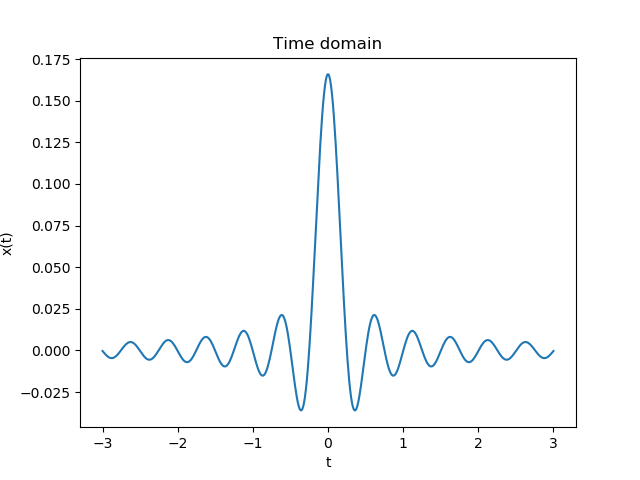
\includegraphics[width=\columnwidth]{time.png}
\caption{Plot of signal in Time domain}
\label{fig:sig_time}
\end{figure}
\begin{figure}[h!]
\centering
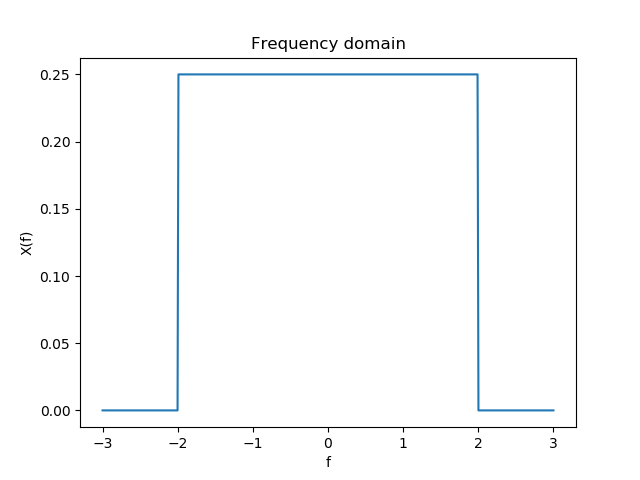
\includegraphics[width=\columnwidth]{freq.png}
\caption{Plot of signal in Frequency domain}
\label{fig:sig_freq}
\end{figure}
\end{document}
